Para mejorar la calidad de la soluci\'on dada por la heur\'istica de b\'usqueda local decidimos usar la metaheur\'istica GRASP (Greedy Randomized Adaptive Search Procedure). Esta metaheur\'istica consiste en generar varias soluciones iniciales (por ejemplo bas\'andose en una heur\'istica greedy) y luego mejorarlas con una b'usqueda local. \\
Nosotros proponemos como soluciones iniciales cuatro \emph{greedies}, cada uno con una condici\'on distinta de decisi\'on del pr\'oximo gimnasio:
\begin{itemize}
    \item El m\'as cercano.
    \item El m\'as lejano.
    \item El m\'as fuerte.
    \item El m\'as d\'ebil.
\end{itemize}

Para que el GRASP sea efectivo cada vez que se puede ir a un gimnasio se elige entre las $n/2$ mejores opciones siendo $n$ la cantidad total de gimnasios. En caso de que haya menos opciones se elegiran entre todos. La elecci\'on se realiza mediante un n\'umero generado pseudoaleatoriamente.

\subsection{Pseudoc\'odigo}

\SetAlgoLined
\SetKwProg{Fn}{Function}{:}{EndFunction}
\begin{algorithm}[H]
	\label{algo: ejercicio4_pseudocodigo}
	\Fn{GRASP}{
	    solucion
		
    	\BlankLine
		\For{desde 0 hasta la cantidad de pokeparadas}{
			\For{cada configuracion de goloso}{
			    solucionParcial $\gets$ calcularGoloso() \\
			    busquedalocal(solucionParcial)\\
			    \If{distancia(solucion)$>$ distancia(solucionParcial)}{
			        solucion $\gets$ solucionParcial
			    }
			}
        }
        return solucion
}
	\caption{Función que implementa la metaheur\'istica GRASP.}
\end{algorithm}


\SetAlgoLined
\SetKwProg{Fn}{Function}{:}{EndFunction}
\begin{algorithm}[H]
	\label{algo: ejercicio4_golosopseudocodigo}
	\Fn{Goloso aleatorio}{
	    \BlankLine
	    		
		\If{hay pokeparadas}{
		    visito el nodo más cercano al primer gimnasio
		}\Else{
		    visito el primer gimnasio
		}
    	\BlankLine
		\While{no haya recorrido todos los gimnasios}{
		    \If{hay gimnasios a los que pueda ir}{
		        ordeno la lista de gimnasios posibles por distancia al nodo actual o cantidad de pociones segun corresponda \\
		        genero un numero pseudoaleatorio entre 0 y la cantidad de gimnasios posibles exclusive \\
		        visito gimnasios\_posibles[random]
		    }\Else{
		        \If{hay pokeparadas sin visitar}{
		            visito la pokeparada más cercana al ultimo nodo visitado
		        }\Else{
		            \Return no existe solucion
		        }
		    }
		}
        \Return la lista con todos los nodos visitados
    }
	\caption{Función que implementa la creaci\'on de la soluci\'on inicial.}
\end{algorithm}


\subsection{Cota de complejidad}
Primero veamos que el goloso para generar la soluci\'on inicial cuesta $O(n^2+(mlog(m))^2))$ con $n$ la cantida de paradas y $m$ la cantidad de gimnasios. La guarda de la l\'inea 2 cuesta $O(1)$ ya que lo representamos con un vector a las pokeparadas. Cualquiera de las dos bifurcaciones cuesta $O(1)$ ya que se agrega un entero al final de una lista. Luego se realizamos un ciclo while, cuyo peor caso es recorrer todas las pokeparadas y, por supuesto, todos los gimnasios. La evaluaci\'on de la guarda cuesta $O(1)$ ya que utilizamos un contador de gimnasios visitados. Despu\'es, en la l\'inea 9 para verificar esa condici\'on recorremos todos los gimnasios y validamos que se cuente con las pociones suficientes para atacarlo y que no lo hayamos visitado a\'un, esto cuesta $O(m)$. La rama verdadera del if es $O(mlog(m))$ ya que ordenar cuesta $O(mlog(m))$ porque en peor caso tengo todos los gimnasios, generar el n\'umero pseudoaleatorio es $O(1)$ y agregar un entero a una lista tambi\'en. En cambio la rama falsa es $O(n)$ ya que se recorren todas las pokeparadas para encontrar la m\'as cercana (en caso de que hay alguna sin visitar). \\
Recapitulando en el ciclo while hay 2 casos, cuando se visita una pokeparada es $O(n)$ y cuando se visita un gimnasio es $O(mlog(m))$, dado que en peor caso nuestro ciclo se ejecuta $O(n+m)$ veces la complejidad total es $O(n^2+(mlog(m))^2))$.

Comencemos analizando el cuerpo del ciclo for de la l\'inea 4. El c\'alculo del goloso de la l\'inea 5 cuesta $O(n^2+(mlog(m))^2)$, la b\'usqueda local de la l\'inea 6 cuesta $O(max(n^4,m^4))$, la guarda de la l\'inea 6 se puede computar en $O(n+m)$ ya que calcular la distancia de un camino es $O(n+m)$ y luego se realiza una comparaci\'on de enteros. Por \'ultimo se copia un vector a otro que tambi\'en cuesta $O(n+m)$. En total el cuerpo de ese for cuesta $O(max(n^4,m^4))$ ya que s\'olo hay 4 configuraciones posibles para nuestro goloso. El ciclo for de la linea 3 hace que nuestro algoritmo tenga complejidad $O(max(n^5,m^5)$ ya que hay $O(n)$ paradas en total.

\subsection{Experimentaci\'on}

Para esta heur\'istica propusimos los siguientes experimentos:

\begin{itemize}

\item Paradas y Gimnasios: Si el enfoque est\'a en la cantidad de nodos se ve que el tiempo de ejecuci\'on pareciera tener una tendencia menor o igual a la complejidad teórica.

\begin{figure}[H]
	\begin{center}
		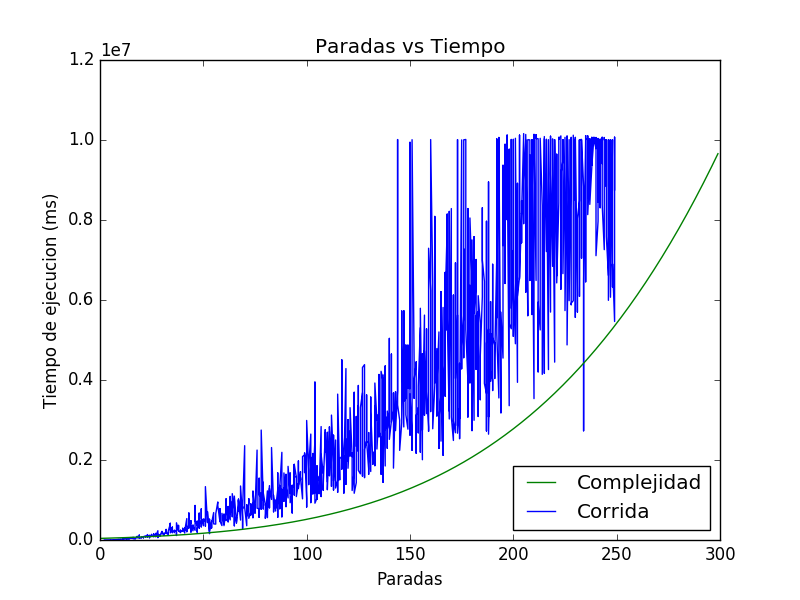
\includegraphics[width=0.7\textwidth]{img/ejercicio4/ParadasTiempos.png}
		\caption{}
		\label{fig: Paradas}
	\end{center}
\end{figure}
\begin{figure}[H]
	\begin{center}
		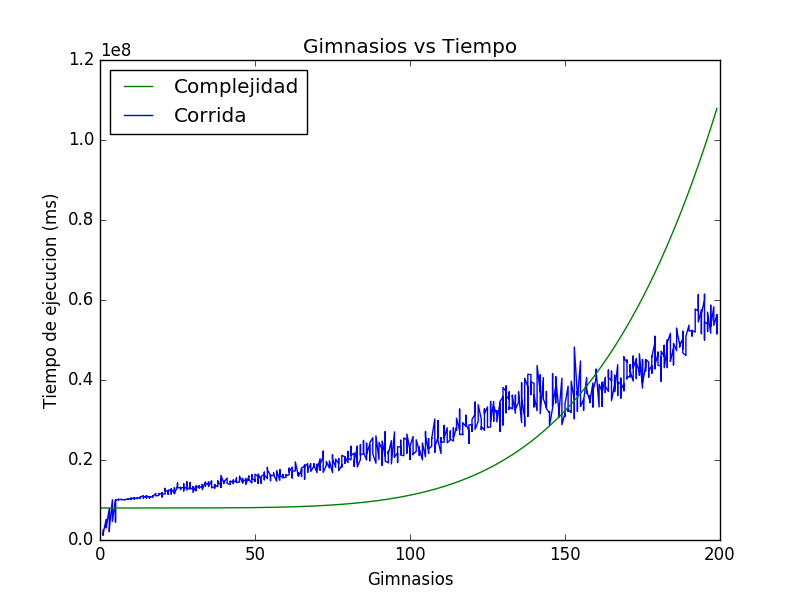
\includegraphics[width=0.7\textwidth]{img/ejercicio4/GimnasiosTiempos.png}
		\caption{}
		\label{fig: Gimnasios}
	\end{center}
\end{figure}


\item Gimnasios: 

Es obvio que si se aumenta la cantidad de gimnasios el tiempo de ejecuci\'on va a aumentar pero lo que queremos mostrar es que si se aumenta la cantidad de nodos obligatorios para el camino el tiempo de ejecuci\'on aumenta dado que a la fuerza tiene que construir un camino m\'as largo. Es importante aclarar que para este experimento tuvimos en cuenta que siempre haya alguna soluci\'on posible, sencillamente se fij\'o la cantidad de nodos totales en 20 y se vari\'o la cantidad de gimnasios. Los casos en los cuales no hay soluci\'on posible no son muy interesantes dado que los algoritmos golosos no iban a devolver una soluci\'on entonces las b\'usquedas locales no se iban a ejecutar.


\begin{figure}[H]
	\begin{center}
		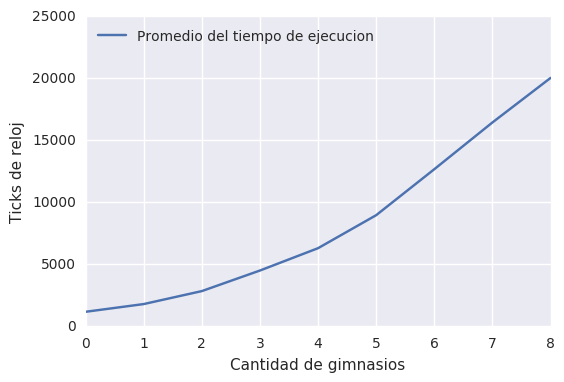
\includegraphics[width=0.7\textwidth]{img/ejercicio4/gimnasios.png}
		\caption{}
		\label{fig: ej4_gimnasios}
	\end{center}
\end{figure}

\item Capacidad de la mochila: 

\begin{figure}[H]
	\begin{center}
		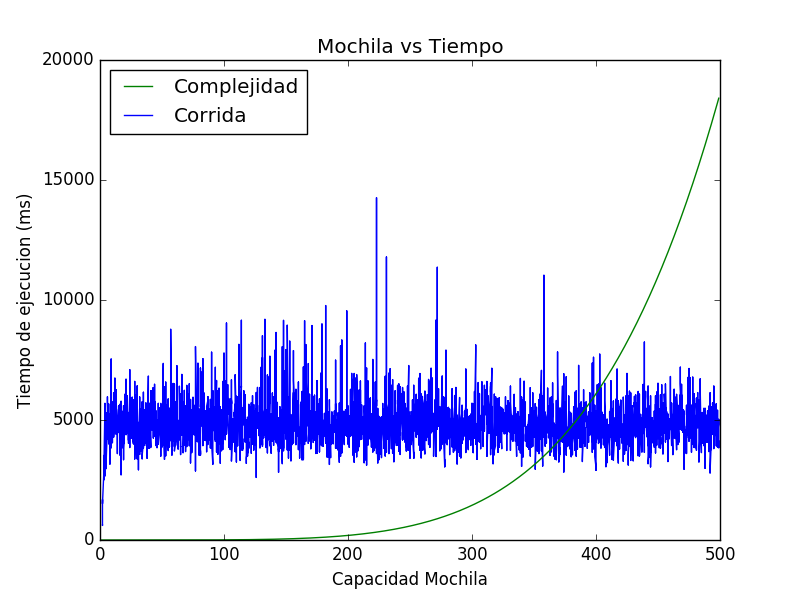
\includegraphics[width=0.7\textwidth]{img/ejercicio4/MochilaTiempos.png}
		\caption{}
		\label{fig: ej4_mochila}
	\end{center}
\end{figure}

En este gr\'afico podemos ver que aumentar la capacidad de la mochila no genera un aumento en el tiempo de ejecuci\'on, inclusive se aprecia que sigue la tendencia nula de una función constante . El rol de la capacidad de la mochila es m\'as que nada para decidir si hay una soluci\'on posible o no, aunque tambi\'en influye levente en la cantidad de pokeparadas visitadas en el camino.

\item Calidad: 

Vemos la diferencia absoluta entre la distancia exacta y la calculada con grasp variando la capacidad de la mochila y luego variando la cantidad de paradas:
\begin{figure}[H]
	\begin{center}
		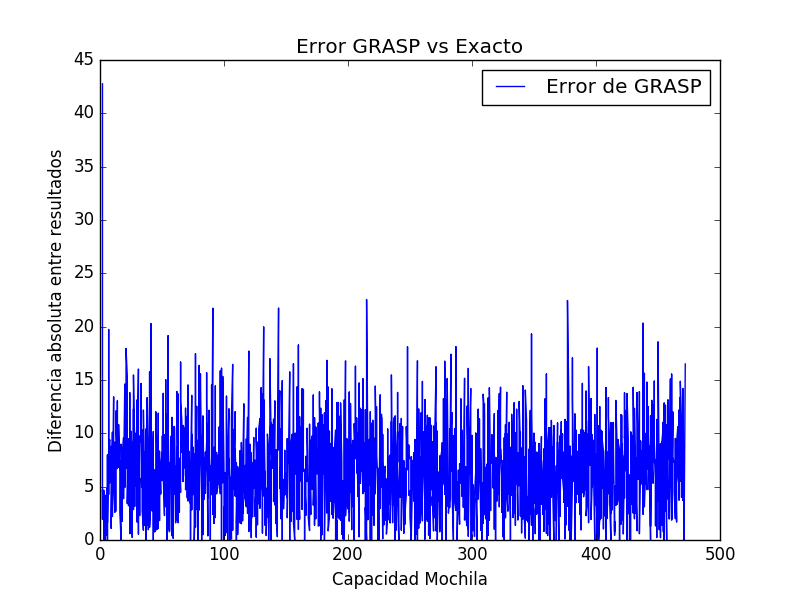
\includegraphics[width=0.7\textwidth]{img/ejercicio4/CalidadMochilas.png}
		\caption{}
		\label{fig: ej4_gimnasios}
	\end{center}
\end{figure}

\begin{figure}[H]
	\begin{center}
		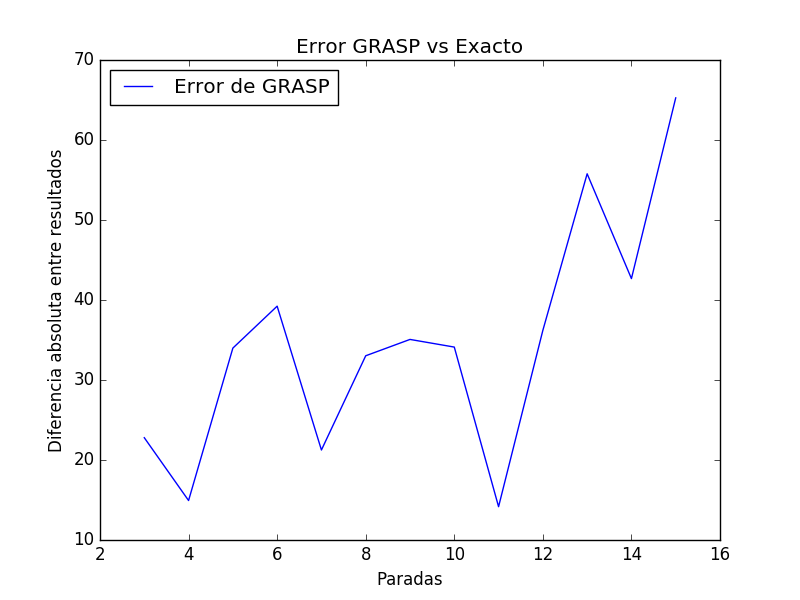
\includegraphics[width=0.7\textwidth]{img/ejercicio4/CalidadPokes.png}
		\caption{}
		\label{fig: ej4_mochila}
	\end{center}
\end{figure}

En el caso de variar la mochila, se ve como el error es constante sobre la capacidad de la mochila.\newline
En el segundo gráfico tenemos pocos nodos como para sacar una conclusión
\end{itemize}

